\chapter{Optimizing LLMs for Retrieval-Augmented Generation}
\label{ch:rag}

\section{Introduction and Motivation}
\label{sec:rag_intro}

Retrieval-Augmented Generation (RAG) has emerged as a critical paradigm for enterprise knowledge management, enabling Large Language Models to provide accurate, contextually grounded responses by incorporating external knowledge sources~\cite{lewis2020rag}. By combining dense retrieval mechanisms with generative models, RAG addresses fundamental limitations of parametric LLMs---namely, their tendency to hallucinate~\cite{huang2023hallucination} and inability to access current or organization-specific information.

However, deploying RAG systems effectively requires careful optimization across multiple dimensions: model selection, retrieval configuration, generation parameters, and evaluation methodology. This chapter synthesizes findings from three accepted publications to establish comprehensive optimization guidelines for enterprise RAG deployment:

\begin{enumerate}[leftmargin=*]
    \item \textbf{Evaluation of Orca 2 for RAG}~\cite{huang2024orca2rag}: Comparative assessment of model performance on RAG benchmarks (PAKDD 2024 Workshops)
    \item \textbf{Performance Analysis of Llama 2}~\cite{huang2024llama2}: In-context learning evaluation across multiple LLMs (IEEE CAI 2024)
    \item \textbf{RAP Metric}~\cite{huang2025rap}: Novel evaluation metric addressing repetition in open-source LLM outputs (NAACL 2025)
\end{enumerate}

The research presented in this chapter addresses the first research question (RQ1): \textit{How can RAG systems be optimized to improve response quality while addressing critical issues such as content repetition in open-source LLMs?} The findings establish foundations that inform subsequent chapters: the evaluation methodology developed here informs the reliability metrics for agentic systems (Chapter~\ref{ch:agentic}), while the model selection insights guide edge deployment strategies (Chapter~\ref{ch:strategies}).

The chapter is organized as follows: Section~\ref{sec:rag_methodology} presents our experimental methodology including datasets, models, and evaluation frameworks. Section~\ref{sec:rag_comparative} details comparative evaluation results demonstrating open-source model competitiveness. Section~\ref{sec:rag_rap} introduces the Repetition-Aware Performance metric and its application to hyperparameter optimization. Section~\ref{sec:rag_guidelines} synthesizes practical deployment guidelines.

\section{Methodology}
\label{sec:rag_methodology}

\subsection{RAG System Architecture}

Our experimental RAG system follows a standard architecture comprising document processing, retrieval, and generation components (Figure~\ref{fig:rag_architecture}), consistent with the framework established by~\citet{gao2023rag_survey}.

\begin{figure}[htbp]
    \centering
    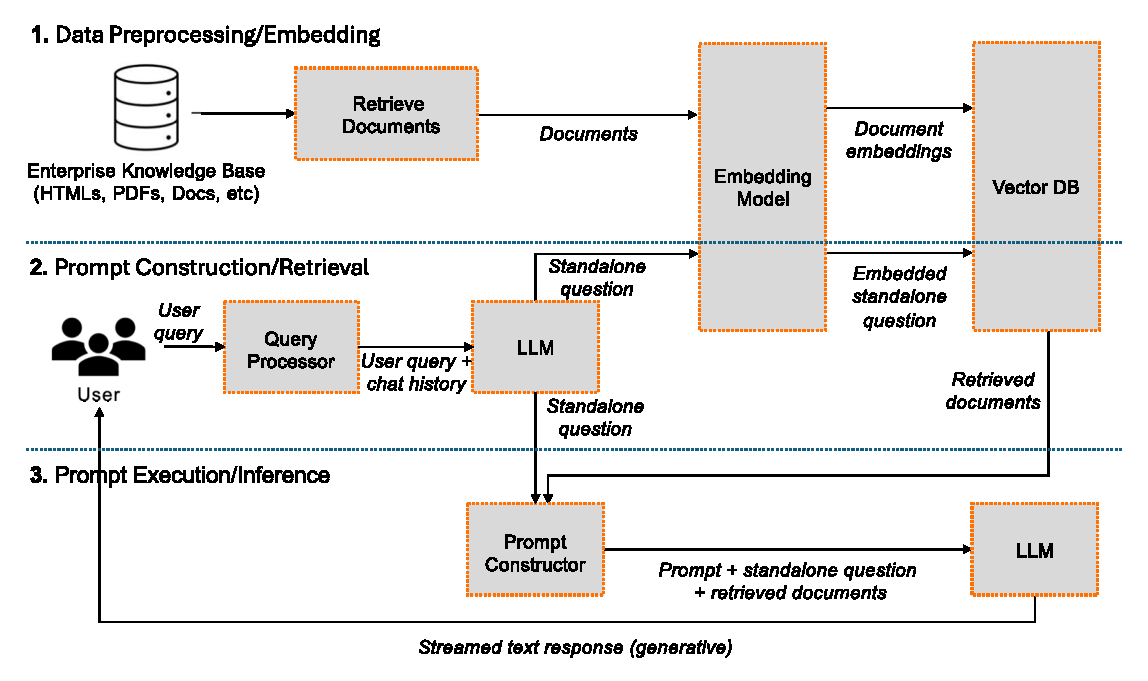
\includegraphics[width=1\textwidth]{figures/RAG.eps}    
    \caption{Overview of the RAG system architecture used in our experiments.}
    \label{fig:rag_architecture}
\end{figure}

\subsubsection{Document Processing}

Documents are processed through the following pipeline:

\begin{enumerate}[leftmargin=*]
    \item \textbf{Text Extraction:} PDF documents are parsed using specialized libraries to extract text while preserving structural information.
    
    \item \textbf{Chunking:} Documents are segmented into chunks of approximately 500 tokens with 50-token overlap to maintain context continuity.
    
    \item \textbf{Embedding:} Text chunks are encoded using the HuggingFace Instructor model~\cite{su2023instructor}, generating 768-dimensional dense vectors.
    
    \item \textbf{Indexing:} Embeddings are stored in FAISS~\cite{johnson2019faiss} for efficient similarity search.
\end{enumerate}

\subsubsection{Retrieval Configuration}

For each user query, the retrieval component:
\begin{itemize}[leftmargin=*]
    \item Encodes the query using the same embedding model
    \item Performs approximate nearest neighbor search to identify top-$k$ relevant chunks ($k=10$ in our experiments)
    \item Returns retrieved chunks as context for generation
\end{itemize}

\subsubsection{Conversational Retrieval Chain}

We employ LangChain's ConversationalRetrievalChain~\cite{langchain2024} for multi-turn interactions. The chain operates in three phases:

\begin{enumerate}[leftmargin=*]
    \item \textbf{Standalone Question Generation:} Synthesizes a context-independent question from chat history and current query
    \item \textbf{Document Retrieval:} Retrieves relevant context using the standalone question
    \item \textbf{Response Generation:} Generates the final response conditioned on retrieved context
\end{enumerate}

This architecture serves as the foundation for more complex multi-agent systems presented in Chapter~\ref{ch:agentic}, where retrieval and generation are orchestrated across specialized agents.

\subsection{Evaluation Datasets}

\subsubsection{PCI DSS Dataset}

For RAG-focused experiments, we utilize documents from the Payment Card Industry Data Security Standard (PCI DSS) version 4.0. This dataset comprises 13 PDF documents obtained from the PCI Security Standards Council, covering security requirements for organizations handling payment card data.

The domain-specific nature of PCI DSS demands accurate technical retrieval, concise synthesis of requirements, and context-aware compliance guidance.

Our evaluation queries focus on:
\begin{enumerate}[leftmargin=*]
    \item Basic definitional questions (``What's PCI DSS?'')
    \item Comparative analysis (``Changes from version 3.2.1 to 4.0'')
    \item Technical deep-dives (``New vulnerability assessment requirements'')
    \item Follow-up clarifications (``More on penetration testing'')
\end{enumerate}

\subsubsection{MS MARCO Dataset}

For broader in-context learning evaluation, we utilize a subset of the MS MARCO dataset~\cite{bajaj2016msmarco}. We curated 500 queries with well-formed answers across five categories:

\begin{table}[htbp]
\centering
\caption{MS MARCO Evaluation Dataset Composition}
\label{tab:msmarco_dataset}
\begin{tabular}{@{}lcc@{}}
\toprule
\textbf{Category} & \textbf{Queries} & \textbf{Example} \\
\midrule
LOCATION & 100 & Where is the Eiffel Tower? \\
NUMERIC & 100 & How many states in the US? \\
PERSON & 100 & Who invented the telephone? \\
DESCRIPTION & 100 & What is photosynthesis? \\
ENTITY & 100 & What is the capital of France? \\
\midrule
\textbf{Total} & \textbf{500} & \\
\bottomrule
\end{tabular}
\end{table}

\subsubsection{WebQSP Dataset}

For knowledge-base question answering (KBQA) evaluation, we utilize the WebQSP dataset~\cite{yih2016webqsp}, comprising 1,008 questions with entity-based answers from Wikidata. This dataset enables evaluation of LLM performance on structured knowledge retrieval tasks.

\subsection{Model Selection}

Table~\ref{tab:models_evaluated} summarizes the LLMs evaluated in our experiments, spanning proprietary and open-source alternatives across a range of parameter counts from 2B to 70B.

\begin{table}[htbp]
\centering
\caption{Large Language Models Evaluated}
\label{tab:models_evaluated}
\begin{tabular}{@{}llcl@{}}
\toprule
\textbf{Model} & \textbf{Organization} & \textbf{Parameters} & \textbf{Type} \\
\midrule
GPT-4 & OpenAI & Unknown & Proprietary \\
GPT-3.5-Turbo & OpenAI & Unknown & Proprietary \\
Orca-2-13b & Microsoft & 13B & Open-source \\
Orca-2-7b & Microsoft & 7B & Open-source \\
Llama-2-70b & Meta & 70B & Open-source \\
Llama-2-13b & Meta & 13B & Open-source \\
Llama-2-7b & Meta & 7B & Open-source \\
Llama-3-70b & Meta & 70B & Open-source \\
Llama-3-8b & Meta & 8B & Open-source \\
Gemma-1.1-7b & Google & 7B & Open-source \\
Gemma-1.1-2b & Google & 2B & Open-source \\
Phi-3-mini & Microsoft & 3.8B & Open-source \\
Mistral-7b & Mistral AI & 7B & Open-source \\
\bottomrule
\end{tabular}
\end{table}

\subsection{Evaluation Metrics}

\subsubsection{Generation Quality Metrics}

We employ the RAGAS framework~\cite{es2023ragas} for generation quality assessment:

\textbf{Faithfulness Score (FS):} Measures factual consistency between generated responses and retrieved context:

\begin{equation}
FS = \frac{\text{Number of contextually supported claims}}{\text{Total number of claims in response}}
\end{equation}

\textbf{Answer Relevancy (AR):} Assesses alignment between responses and user queries, computed as the cosine similarity between the original query and questions that the response would answer.

\textbf{Overall Score:} Harmonic mean of Faithfulness and Answer Relevancy:

\begin{equation}
\text{Overall} = \frac{2 \times FS \times AR}{FS + AR}
\end{equation}

\subsubsection{Inference Speed}

Measured as tokens generated per second, capturing practical deployment considerations for real-time applications.

\subsubsection{Answer Quality for In-Context Learning}

For MS MARCO evaluation, we employ:
\begin{itemize}[leftmargin=*]
    \item \textbf{ROUGE-L:} Longest common subsequence-based similarity~\cite{lin2004rouge}
    \item \textbf{BLEU-1:} Unigram precision with brevity penalty~\cite{papineni2002bleu}
\end{itemize}

\subsection{Hardware Configuration}

Experiments were conducted on multiple hardware configurations:

\begin{itemize}[leftmargin=*]
    \item \textbf{Consumer Desktop:} NVIDIA GeForce RTX 4090 (24GB VRAM)
    \item \textbf{Professional Workstation:} NVIDIA A40 (48GB VRAM)
    \item \textbf{High-Performance Server:} NVIDIA L40 (48GB VRAM)
\end{itemize}

This diversity enables evaluation of model performance across typical enterprise hardware tiers, informing the comprehensive hardware benchmarking presented in Chapter~\ref{ch:strategies}.

\section{Comparative Evaluation of LLMs for RAG}
\label{sec:rag_comparative}

\subsection{Generation Quality Results}

Figure~\ref{fig:generation_quality} presents generation quality metrics across evaluated models on the PCI DSS benchmark.

\begin{figure}[htbp]
    \centering
    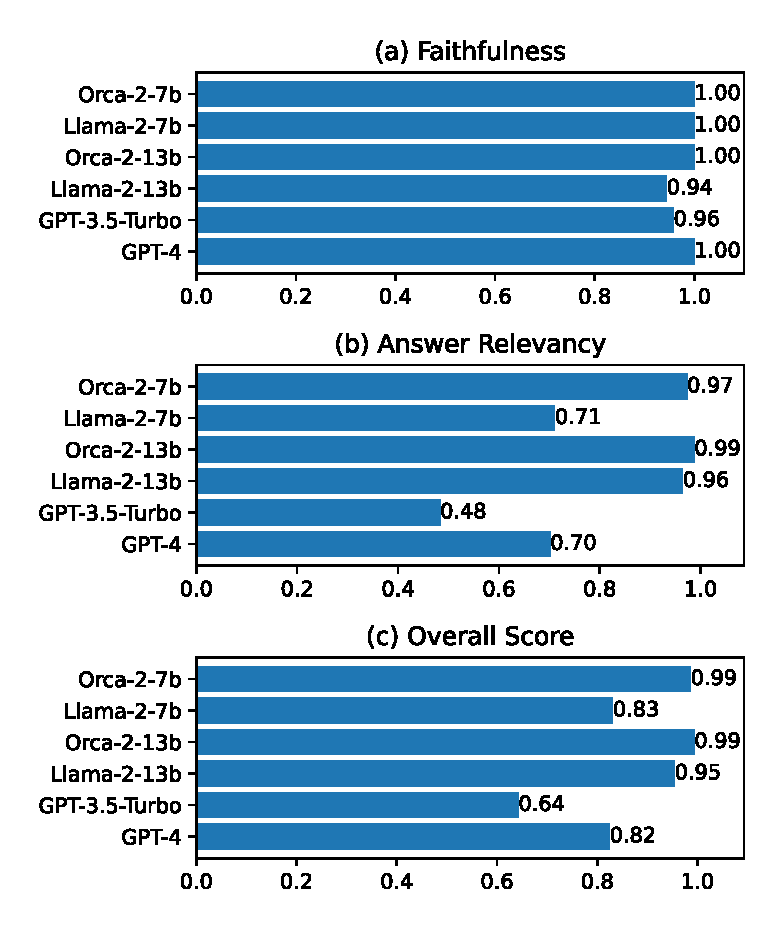
\includegraphics[width=0.9\textwidth]{figures/perf_scores.eps}
    \caption{Comparison of generation quality metrics across LLMs on PCI DSS benchmark.}
    \label{fig:generation_quality}
\end{figure}

Key observations include:

\textbf{Faithfulness:} All models except GPT-3.5-Turbo and Llama-2-13b achieved perfect faithfulness scores (100\%), indicating strong factual consistency with retrieved context. The lower scores for GPT-3.5-Turbo appear attributable to its tendency to rely on parametric knowledge rather than retrieved context.

\textbf{Answer Relevancy:} Orca-2-13b and Orca-2-7b achieved top performance, with scores approaching 99\%. This demonstrates their effectiveness in providing contextually relevant responses aligned with user queries.

\textbf{Overall Score:} Orca-2-13b achieved the highest overall score (99.3\%), followed closely by Orca-2-7b (99.2\%), indicating balanced performance across quality dimensions.

Table~\ref{tab:rag_results_summary} summarizes the quantitative results.

\begin{table}[htbp]
\centering
\caption{RAG Generation Quality Results on PCI DSS Benchmark}
\label{tab:rag_results_summary}
\begin{tabular}{@{}lccc@{}}
\toprule
\textbf{Model} & \textbf{Faithfulness (\%)} & \textbf{Answer Relevancy (\%)} & \textbf{Overall (\%)} \\
\midrule
Orca-2-13b & 100.0 & 98.7 & 99.3 \\
Orca-2-7b & 100.0 & 98.5 & 99.2 \\
GPT-4 & 100.0 & 95.2 & 97.5 \\
Llama-2-7b & 100.0 & 92.1 & 95.9 \\
GPT-3.5-Turbo & 87.3 & 89.8 & 88.5 \\
Llama-2-13b & 91.2 & 85.4 & 88.2 \\
\bottomrule
\end{tabular}
\end{table}

\subsection{Open-Source Model Competitiveness}

A central finding of our evaluation is that properly configured open-source models can match or exceed proprietary alternatives for RAG applications. Orca-2-13b achieved a 99.3\% overall RAGAS score---surpassing GPT-4 (97.5\%) while operating on consumer-grade hardware. This finding challenges the assumption that proprietary models are necessary for high-quality RAG deployment and has significant implications for enterprise cost management and data privacy.

The performance advantage of Orca-2 models appears attributable to their training methodology, which emphasizes learning from complex explanation traces rather than simply imitating larger models~\cite{mitra2023orca}. This training approach produces models that more reliably follow retrieved context rather than defaulting to parametric knowledge---a critical capability for enterprise RAG applications where accuracy must be grounded in organizational documents.

This finding---that smaller, specialized models can outperform larger general-purpose alternatives---recurs throughout this dissertation. In Chapter~\ref{ch:agentic}, we observe similar patterns where qwen2.5:32b matches GPT-4.1 performance for invoice reconciliation, and in Chapter~\ref{ch:strategies}, DeepSeek-R1:32b substantially outperforms DeepSeek-R1:70b on sentiment classification tasks.

\subsection{Inference Speed Analysis}

Figure~\ref{fig:inference_speed} presents inference speed comparisons.

\begin{figure}[htbp]
    \centering
    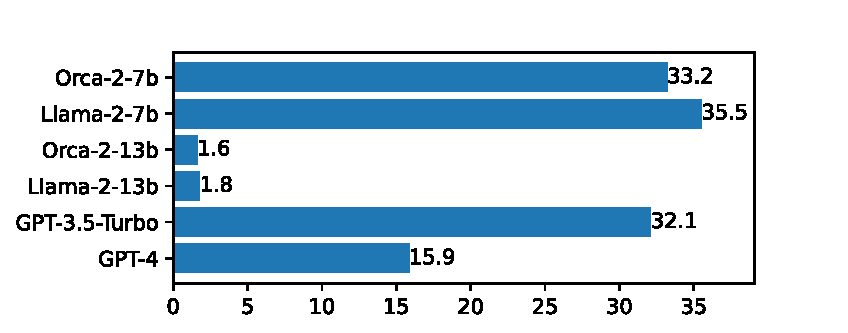
\includegraphics[width=0.9\textwidth]{figures/inference_speed.eps}
    \caption{Inference speed comparison across LLMs on consumer and professional hardware.}
    \label{fig:inference_speed}
\end{figure}

The Orca-2-7b model achieved approximately 33 tokens per second on the RTX 4090, closely matching GPT-3.5-Turbo (32 tokens/sec) and significantly outperforming GPT-4 (16 tokens/sec). This demonstrates that smaller, efficient models can provide competitive throughput on consumer-grade hardware.

Notable observations:
\begin{itemize}[leftmargin=*]
    \item 13B parameter models exhibited slower speeds due to GPU memory constraints
    \item Running Orca-2-13b on the A40 (48GB) improved speed to approximately 15 tokens/sec
    \item Hardware memory capacity significantly impacts larger model performance
\end{itemize}

\subsection{Qualitative Analysis}

Examination of generated responses revealed several patterns:

\textbf{Language Switching:} Orca-2-13b occasionally switched to Spanish after the first question while maintaining high quality scores. This indicates that RAGAS evaluation---utilizing GPT-4-Turbo---assesses quality based on semantics rather than language consistency.

\textbf{Standalone Question Generation:} Models exhibited varying quality in generating standalone questions for retrieval. Orca-2-7b sometimes produced generic questions, while other models maintained query specificity.

\textbf{Context Utilization:} GPT-3.5-Turbo and GPT-4 occasionally ignored retrieved context in favor of parametric knowledge, explaining their lower faithfulness scores in some scenarios. This behavior is particularly problematic for enterprise applications where responses must be grounded in organizational documents.

\section{The Repetition-Aware Performance Metric}
\label{sec:rag_rap}

When optimizing a RAG system, it is crucial to employ evaluation metrics that can effectively guide both system development and automated hyperparameter tuning. Standard metrics for QA or text generation (e.g., accuracy, F1, BLEU) capture how well the generated content aligns with the ground truth but fail to account for issues like redundancy or verbosity. In open-source LLMs---particularly those not rigorously RLHF-tuned for conciseness---repetitive outputs are common~\cite{fu2020repetition}. For instance, a model might repeat a sentence from the context multiple times or generate unnecessarily long sequences of non-word characters, such as repeated newlines. Such behavior not only degrades user experience but can also indirectly reduce accuracy if key information becomes obscured by repetitive content. This is particularly problematic in tasks requiring coherent and contextually relevant responses, such as conversational chatbots and---as we demonstrate in Chapter~\ref{ch:agentic}---multi-agent systems where output quality directly impacts downstream component reliability.

To address this, the \textit{repetition penalty parameter} (RPP) is employed during the sampling process to reduce redundant outputs by penalizing previously seen tokens~\cite{keskar2019ctrl}. While effective, excessive application of RPP can result in incomplete or fragmented responses, ultimately diminishing user satisfaction.

To address this issue, we introduced the \emph{Repetition-Aware Performance} (RAP) metric in our NAACL 2025 paper~\cite{huang2025rap}. That work investigates the relationship between the repetition penalty parameter (RPP) and its effect on generated text. While parameters like \textit{temperature} and \textit{top-k sampling} are typically optimized via random or grid search, these approaches are inadequate for tuning RPP because conventional metrics, such as precision and BLEU scores~\cite{papineni2002bleu}, fail to account for repetition.

To address this, we propose a metric called \textbf{R}epetition-\textbf{A}ware \textbf{P}erformance (RAP), which quantifies repetition and penalizes it in the model's performance evaluation, allowing for the tuning of RPP. 
Figure~\ref{fig:hook} illustrates tuning RPP for Llama-3-8B using the original evaluation metrics (Original) and our proposed metric. For the WebQSP dataset~\cite{yih2016webqsp}, repetition ratio (RR) is reduced by 93.1\% but the performance only drops by 3.7\%. For the MS MARCO dataset~\cite{bajaj2016msmarco}, RR drops by 73.9\% with only 3.7\% of performance drop. Tuning RPP using RAP can significantly reduce the RR with minimal performance loss. 

\begin{figure}[htbp]
    \centering
    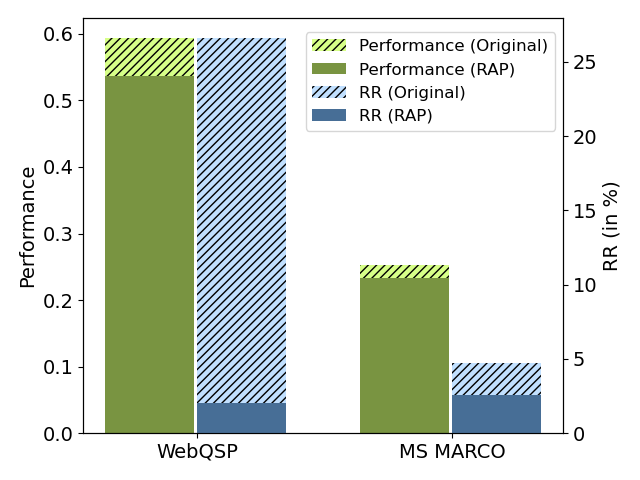
\includegraphics[width=.7\linewidth]{rap_image/chart_00_w_legend_Meta-Llama-3-8B-Instruct(RAG - Generic Prompt)_2.png}
    \caption{Best performance (F1 for WebQSP, BERT-F1 for MS MARCO) when tuning RPP using original evaluation metrics (Original) and our proposed repetition-aware performance metric (RAP). RAP helps find RPP values that minimally reduce performance while significantly lowering repetition ratio (RR). Result is from Llama-3-8B (RAG-Generic Prompt).}
    \label{fig:hook}
\end{figure}

To compute RAP, we introduce an efficient algorithm called ReDA---Repetition Detection Algorithm---designed to identify all repeating patterns, including non-word character (NWC) and text repetitions, along with their corresponding repetition lengths. Additionally, we define the repetition ratio (RR), which measures the proportion of repeated content relative to the total text length. RR is applied to penalize the model's performance using a cubic penalty formula, as detailed in Section~\ref{sec:rap_definition}. Figure~\ref{fig:overall} illustrates computing RAP with a running example. Although the accuracy is 100\%, the content contains many repeated elements, resulting in a low RAP score of 24.63\%.

\begin{figure*}[htbp]
    \centering
    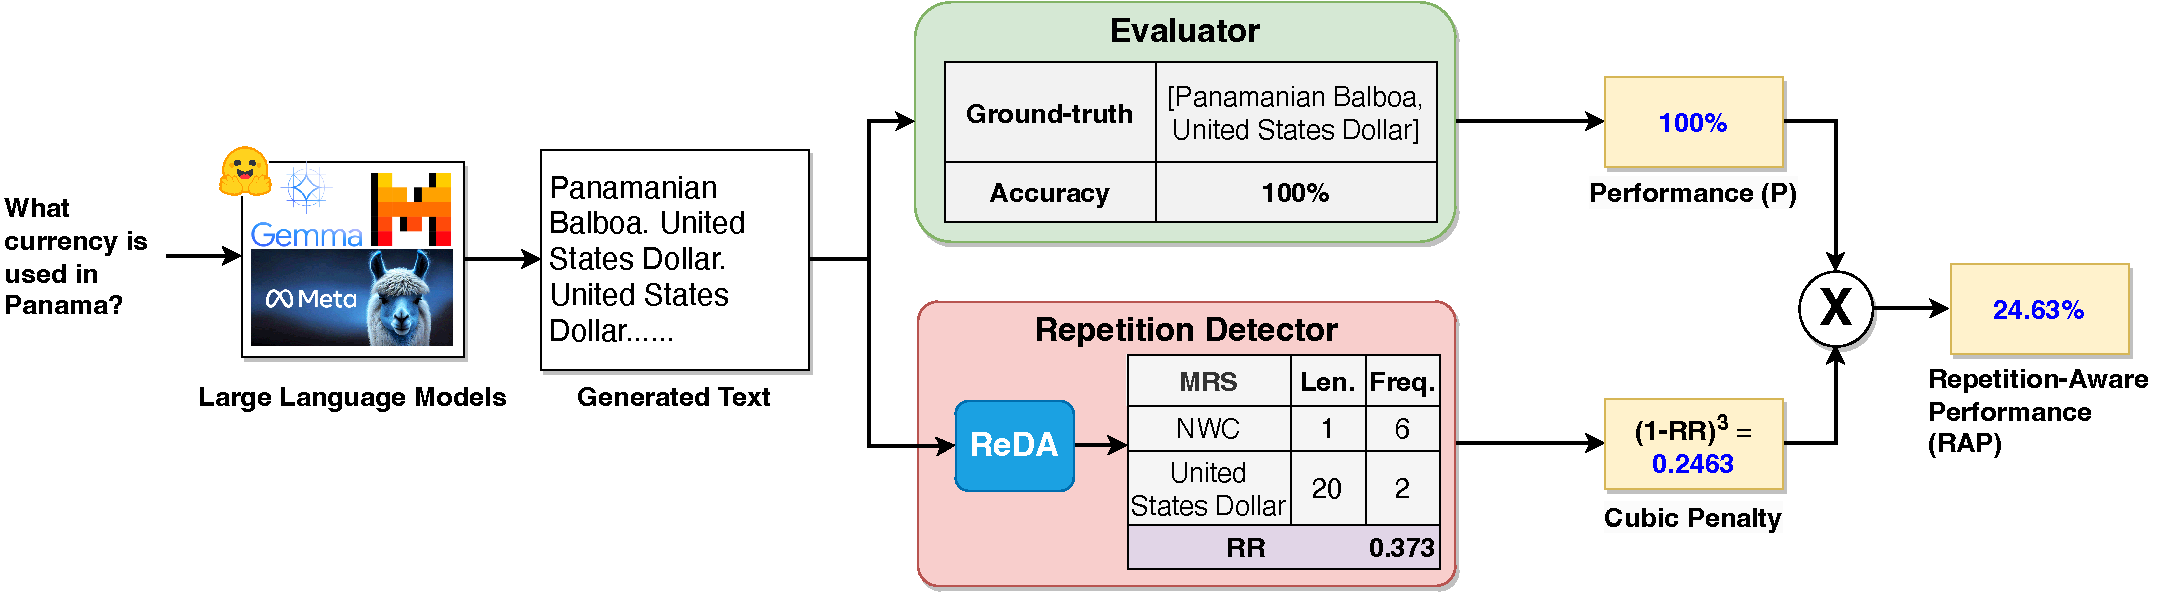
\includegraphics[width=\textwidth]{rap_image/RAPGeT_v3-v5.2.pdf}
    \caption{Overall Methodology: RAP integrates the repetition penalty in the evaluation score. In the example, the generated text contains non-word characters (NWC) repetition and text repetition. After penalization, the accuracy is reduced from 100\% to 24.63\%. ReDA stands for Repetition Detection Algorithm.}
    \label{fig:overall}
\end{figure*}

We conduct experiments on three datasets encompassing question answering (including knowledge base question answering---KBQA---and open-ended QA) and machine translation tasks.
We evaluate twelve open-source LLMs ranging from 2 to 70 billion parameters. 
We also examine the effect of repetition suppression for different prompting strategies including Retrieval-Augmented Generation (RAG)~\cite{lewis2020rag} and non-RAG, combining with generic prompt and chat template.

Our study reveals that increasing RPP typically reduces repetition but often results in performance degradation, highlighting the importance of tuning RPP. The effects of RPP differ across various models, datasets, and prompting techniques. Additionally, we find that using chat templates is effective in reducing repetition for QA tasks. Our experimental results demonstrate that RAP can effectively tune RPP, helping to identify a trade-off value that significantly reduces repetition while minimizing performance loss.
These findings offer insights into optimizing RPP for performance and repetition suppression in open-source LLMs.

\subsection{Repetition Ratio (RR)}
\label{sec:rr_definition}

First, we define the \textbf{Repetition Ratio (RR)} for a set of outputs (e.g., all answers in an evaluation set). The repetition ratio measures the portion of the generated text that is composed of repetitive content. To compute RR, repetition must be detected at both the character level (e.g., excessive whitespace or punctuation) and the word/phrase level. We employ a repetition detection algorithm (ReDA) that identifies two types of repetition:
\begin{itemize}[leftmargin=*]
    \item \textbf{Non-word Character (NWC) Repetition:} Sequences of spaces or other non-alphanumeric characters that are overly long (e.g., multiple newline characters or dashes), indicating that the model is stalling or outputting blank lines.
    \item \textbf{Textual Repetition:} Longer sequences of words that repeat. We search for any substring of length $\geq L$ (a threshold such as 5 characters) that appears at least twice in the output.
\end{itemize}

For each generated output $S$, let $R(S)$ denote the total length (in characters) of all repeated segments identified in $S$ (summing lengths from both NWC and textual repetition). Let $|S|$ be the total length of $S$. Then, the repetition ratio for a single output is defined as:
\[
r(S) = \frac{R(S)}{|S|}.
\]
For an entire set $D$ of outputs, the aggregate repetition ratio is given by:
\begin{equation}
\text{RR}_D = \frac{\sum_{S \in D} R(S)}{\sum_{S \in D} |S|}\,.\label{eq:rr_dataset}
\end{equation}
Here, $\text{RR}_D = 0$ indicates no repetition, while a value of $0.10$ indicates that 10\% of the generated text is redundant.

In practice, $R(S)$ is implemented using regular expressions to detect runs of whitespace, punctuation, and repeated substrings efficiently~\cite{huang2025rap}. Algorithm~\ref{alg:reda} provides pseudocode for the ReDA algorithm, which iteratively removes detected repetitions and sums their lengths.

\begin{algorithm}[htbp]
\caption{Repetition Detection (ReDA)~\cite{huang2025rap}}
\label{alg:reda}
\begin{algorithmic}[1]
\Require Generated text $S$
\Ensure Repetition lengths $L_{\text{NWC}}, L_{\text{text}}, L_{\text{total}}$
\State $L_{\text{NWC}} \gets 0$, $L_{\text{text}} \gets 0$
\State Use regex to find any occurrence of 5 or more non-word characters in a row in $S$
\If{matches found}
    \State Remove these sequences from $S$ and increment $L_{\text{NWC}}$ by the total number of removed characters
\EndIf
\State Use regex to find repeated textual patterns of length $\geq 5$ in $S$
\For{\textbf{each} match of a repeated substring of length $\ell$ in $S$}
    \State $L_{\text{text}} \gets L_{\text{text}} + \ell$ \Comment{Accumulate lengths of repeats}
\EndFor
\State $L_{\text{total}} \gets L_{\text{NWC}} + L_{\text{text}}$
\State \Return $(L_{\text{NWC}}, L_{\text{text}}, L_{\text{total}})$
\end{algorithmic}
\end{algorithm}

\subsection{Defining the RAP Score}
\label{sec:rap_definition}

With $\text{RR}_D$ computed, we define the RAP score for the model's outputs. Let $P$ be the base performance metric of interest (e.g., average F1 score, exact match accuracy, BERT-F1, or COMET, depending on the task). We incorporate a repetition penalty through a function $F(\text{RR}_D)$ that decreases from 1 as $\text{RR}_D$ increases. In our work, we use a cubic penalty for smoothness:
\[
F(\text{RR}) = (1 - \text{RR})^3\,.
\]
The RAP score is then defined as:
\begin{equation}
\text{RAP} = P \times F(\text{RR}_D)\,.\label{eq:rap}
\end{equation}
If the model produces no repetition ($\text{RR}_D = 0$, so $F=1$), then $\text{RAP} = P$. If there is any repetition, then $0 < F < 1$, leading to $\text{RAP} < P$, effectively lowering the performance score in proportion to the repetition. For example, if $\text{RR}_D = 0.1$ (10\% repetition), then $F(0.1) = 0.9^3 \approx 0.729$, meaning the model retains roughly 73\% of its base score under RAP. This approach incentivizes reducing repetition.

RAP is valuable in two ways:
\begin{enumerate}[leftmargin=*]
    \item It can guide hyperparameter tuning (see Section~\ref{sec:rag_opt}). For instance, when tuning the repetition penalty parameter (RPP), using only accuracy might select a configuration with higher accuracy but excessive redundancy. RAP leads to choosing an RPP that balances performance and conciseness.
    \item It allows for holistic model comparisons. In our experiments, while larger models had higher raw performance, some smaller models achieved comparable RAP scores due to reduced redundancy---an important insight for enterprise deployments.
\end{enumerate}

It is important to ensure that RAP does not excessively penalize necessary repetitions. In some contexts, repeating critical instructions---such as ``Please read carefully. Please read carefully.''---is essential for ensuring emphasis and clarity. Our ReDA algorithm is designed to detect only excessive or verbose repetitions; small amounts of repetition yield a penalty factor close to 1. In practice, we found that RAP correlates well with human judgments of answer quality when redundancy is taken into account.

\subsection{Experimental Settings}
\label{sec:rap_experiments}

\textbf{Datasets.} We conduct our experiments on three datasets: WebQSP~\cite{yih2016webqsp} and MS MARCO~\cite{bajaj2016msmarco} for question answering (QA), and MAC~\cite{huang2025translation} for Chinese-English machine translation (MT). The test sets contain 1,008, 500, and 1,133 questions, respectively. For WebQSP, we crawl relevant Wikipedia articles and retrieve the 8 most pertinent document chunks per question to form RAG prompts. We also adopt Gemini-1.0-Pro to evaluate the knowledge base QA (KBQA) task, where ground-truth answers consist of lists of entities rather than free-form text.

\paragraph{Cross-Task Validation with Machine Translation.}
While this chapter focuses primarily on RAG optimization for question answering, we include machine translation (MT) experiments to demonstrate the generalizability of the RAP metric. The repetition problem is not unique to RAG-based QA---it manifests across diverse generation tasks. Validating RAP on MT establishes its applicability as a general-purpose evaluation metric for open-source LLMs, regardless of whether retrieved context is involved. This cross-task validation strengthens confidence in RAP's utility for enterprise deployments spanning multiple use cases. The MT findings presented here lay groundwork for the comprehensive translation evaluation in Chapter~\ref{ch:strategies}, where we introduce additional metrics (Translation Completeness Ratio, Characters per Second) for deployment-oriented assessment.

\textbf{Open-Source LLMs.} This study evaluates a diverse set of open-source large language models (LLMs) for question answering (QA) and machine translation (MT) tasks. For QA, we assess nine models: Llama-2 (7B, 13B, 70B), Llama-3 (8B, 70B), Gemma-1.1 (2B, 7B), Phi-3-mini (3.8B), and Mistral-7B. For MT, we evaluate three models: Phi-3.5-mini (3.8B), Mistral-7B, and Llama-3.1-70B. Table~\ref{tab:ai_models} provides an overview of these models---including their companies, model names, Hugging Face identifiers, and the tasks on which they were evaluated. This selection spans a broad range of model sizes and architectures, representing the state of the art in open-source LLM development and commercial use.

\begin{table*}[htbp]
\caption{Overview of Large Language Models and Their Specifications by Task}
\label{tab:ai_models}
\centering
\resizebox{.85\textwidth}{!}{
\begin{tabular}{l|l|l|l}
\toprule
\textbf{Company} & \textbf{Model Name} & \textbf{Hugging Face Model ID} & \textbf{Task} \\
\midrule
\multirow{6}{*}{Meta} 
& Llama-2-7B & meta-llama/Llama-2-7b-chat & QA \\
& Llama-2-13B & meta-llama/Llama-2-13b-chat & QA \\
& Llama-2-70B & meta-llama/Llama-2-70b-chat & QA \\
& Llama-3-8B & meta-llama/Meta-Llama-3-8B-Instruct & QA \\
& Llama-3-70B & meta-llama/Meta-Llama-3-70B-Instruct & QA \\
& Llama-3.1-70B & shenzhi-wang/Llama3.1-70B-Chinese-Chat & MT \\
\midrule
\multirow{2}{*}{Microsoft} 
& Phi-3-mini & microsoft/Phi-3-mini-128k-instruct & QA \\
& Phi-3.5-mini & microsoft/Phi-3.5-mini-instruct & MT \\
\midrule
\multirow{2}{*}{Google} 
& Gemma-1.1-2B & google/gemma-1.1-2b-it & QA \\
& Gemma-1.1-7B & google/gemma-1.1-7b-it & QA \\
\midrule
\multirow{2}{*}{Mistral AI} 
& Mistral-7B-v0.2 & mistralai/Mistral-7B-Instruct-v0.2 & QA \\
& Mistral-7B-v0.3 & shenzhi-wang/Mistral-7B-v0.3-Chinese-Chat & MT \\
\bottomrule
\end{tabular}
}
\end{table*}

\textbf{Automating QA and MT Tasks with LLMs.} We developed a Python script leveraging the HuggingFace Transformers library~\cite{wolf2020transformers} to automate evaluation across all models and datasets. For QA, a repetition penalty (RP) ranging from 1.0 to 1.3 (in increments of 0.02) was applied; for MT, an RP range of 1.0 to 1.1 was used. To ensure consistency and reproducibility, the temperature was set to 0 and \texttt{top\_p} was fixed at 0.95.

\textbf{Prompt Templates.} To explore the impact of prompting strategies, we implemented three QA prompt templates: (1) \textit{RAG - Generic Prompt} (RAG-GP): a uniform template applied to all models; (2) \textit{RAG - Chat Template} (RAG-CT): LangChain's default template adapted to each LLM's chat format, preserving core content; and (3) \textit{Non-RAG}: a template simulating a single-turn conversation in the LLM's native chat format. For MT, we employed two templates: (1) \textit{MT - Generic Prompt} (MT-GP): a basic template applied uniformly; and (2) \textit{MT - Chat Template} (MT-CT): a template customized to each LLM's chat format.

The following listings describe the prompt templates used in our experiments.

\begin{lstlisting}[caption={RAG - Generic Prompt template for question answering. The placeholders \texttt{\{question\}} and \texttt{\{context\}} are filled with the question and retrieved data, respectively.},label={list:rag-generic},basicstyle=\small\ttfamily,breaklines=true,frame=single]
Use the following pieces of context to answer the question at the end. If you don't know the answer, just say that you don't know, don't try to make up an answer.
{context}
Question: {question}
Helpful Answer:
\end{lstlisting}

\begin{lstlisting}[caption={Non-RAG prompt template for question answering with Llama-3 models. The placeholder \texttt{\{question\}} is filled with the question.},label={list:non-rag},basicstyle=\small\ttfamily,breaklines=true,frame=single]
<|begin_of_text|>
<|start_header_id|>system<|end_header_id|>
You are a chatbot having a conversation with a human.
<|eot_id|>
<|start_header_id|>user<|end_header_id|>
{question}
<|eot_id|>
<|start_header_id|>assistant<|end_header_id|>
\end{lstlisting}

\begin{lstlisting}[caption={RAG - Chat Template for Llama-3 models. The placeholders \texttt{\{question\}} and \texttt{\{context\}} are filled with the question and retrieved data, respectively.},label={list:rag-chat},basicstyle=\small\ttfamily,breaklines=true,frame=single]
<|begin_of_text|>
<|start_header_id|>system<|end_header_id|>
You are a chatbot having a conversation with a human.
<|eot_id|>
<|start_header_id|>user<|end_header_id|>
Use the following pieces of context to answer the question at the end. If you don't know the answer, just say that you don't know, don't try to make up an answer.
{context}
Question: {question}
<|eot_id|>
<|start_header_id|>assistant<|end_header_id|>
\end{lstlisting}

\begin{lstlisting}[caption={Machine Translation - Generic Prompt (MT-GP) for all models. The placeholder \texttt{\{input\}} is filled with the Chinese sentence from the MAC testing set.},label={list:mt-generic},basicstyle=\small\ttfamily,breaklines=true,frame=single]
You will be given a Chinese sentence to translate. If it is an incomplete sentence, or if you are unsure about the meaning, simply copy the input text as your output. Do not output any additional sentences, such as explanations or reasoning.
Chinese: {input}
\end{lstlisting}

\begin{lstlisting}[caption={Machine Translation - Chat Template (MT-CT) for Llama-3 models. The placeholder \texttt{\{input\}} is filled with the Chinese sentence from the MAC testing set.},label={list:mt-chat},basicstyle=\small\ttfamily,breaklines=true,frame=single]
<|begin_of_text|>
<|start_header_id|>system<|end_header_id|>
You are a helpful assistant that translates Chinese to English.
<|eot_id|>
<|start_header_id|>user<|end_header_id|>
You will be given a Chinese sentence to translate. If it is an incomplete sentence, or if you are unsure about the meaning, simply copy the input text as your output. Do not output any additional sentences, such as explanations or reasoning.
Chinese: {input}
<|eot_id|>
<|start_header_id|>assistant<|end_header_id|>
\end{lstlisting}

\textbf{Evaluation Metrics.} For WebQSP, we report precision, recall, and F1 scores. For MS MARCO, we use BERTScore~\cite{zhang2020bertscore} (with the deberta-xlarge-mnli model) and report the average F1 score (\textit{BERT-F1}). For MAC, we employ the Crosslingual Optimized Metric for Evaluation of Translation (COMET)~\cite{rei2022comet}, which leverages contextual embeddings from pretrained language models to assess translation quality. In addition, we report the repetition ratio (Equation~\ref{eq:rr_dataset}) and the RAP scores (Section~\ref{sec:rap_definition}), which incorporate a penalty for repetition into the performance metrics.

\subsection{Impact of RPP on Repetition and Performance}
\label{subsec:impact_of_rpp}

\begin{figure*}[htbp]
    \centering
    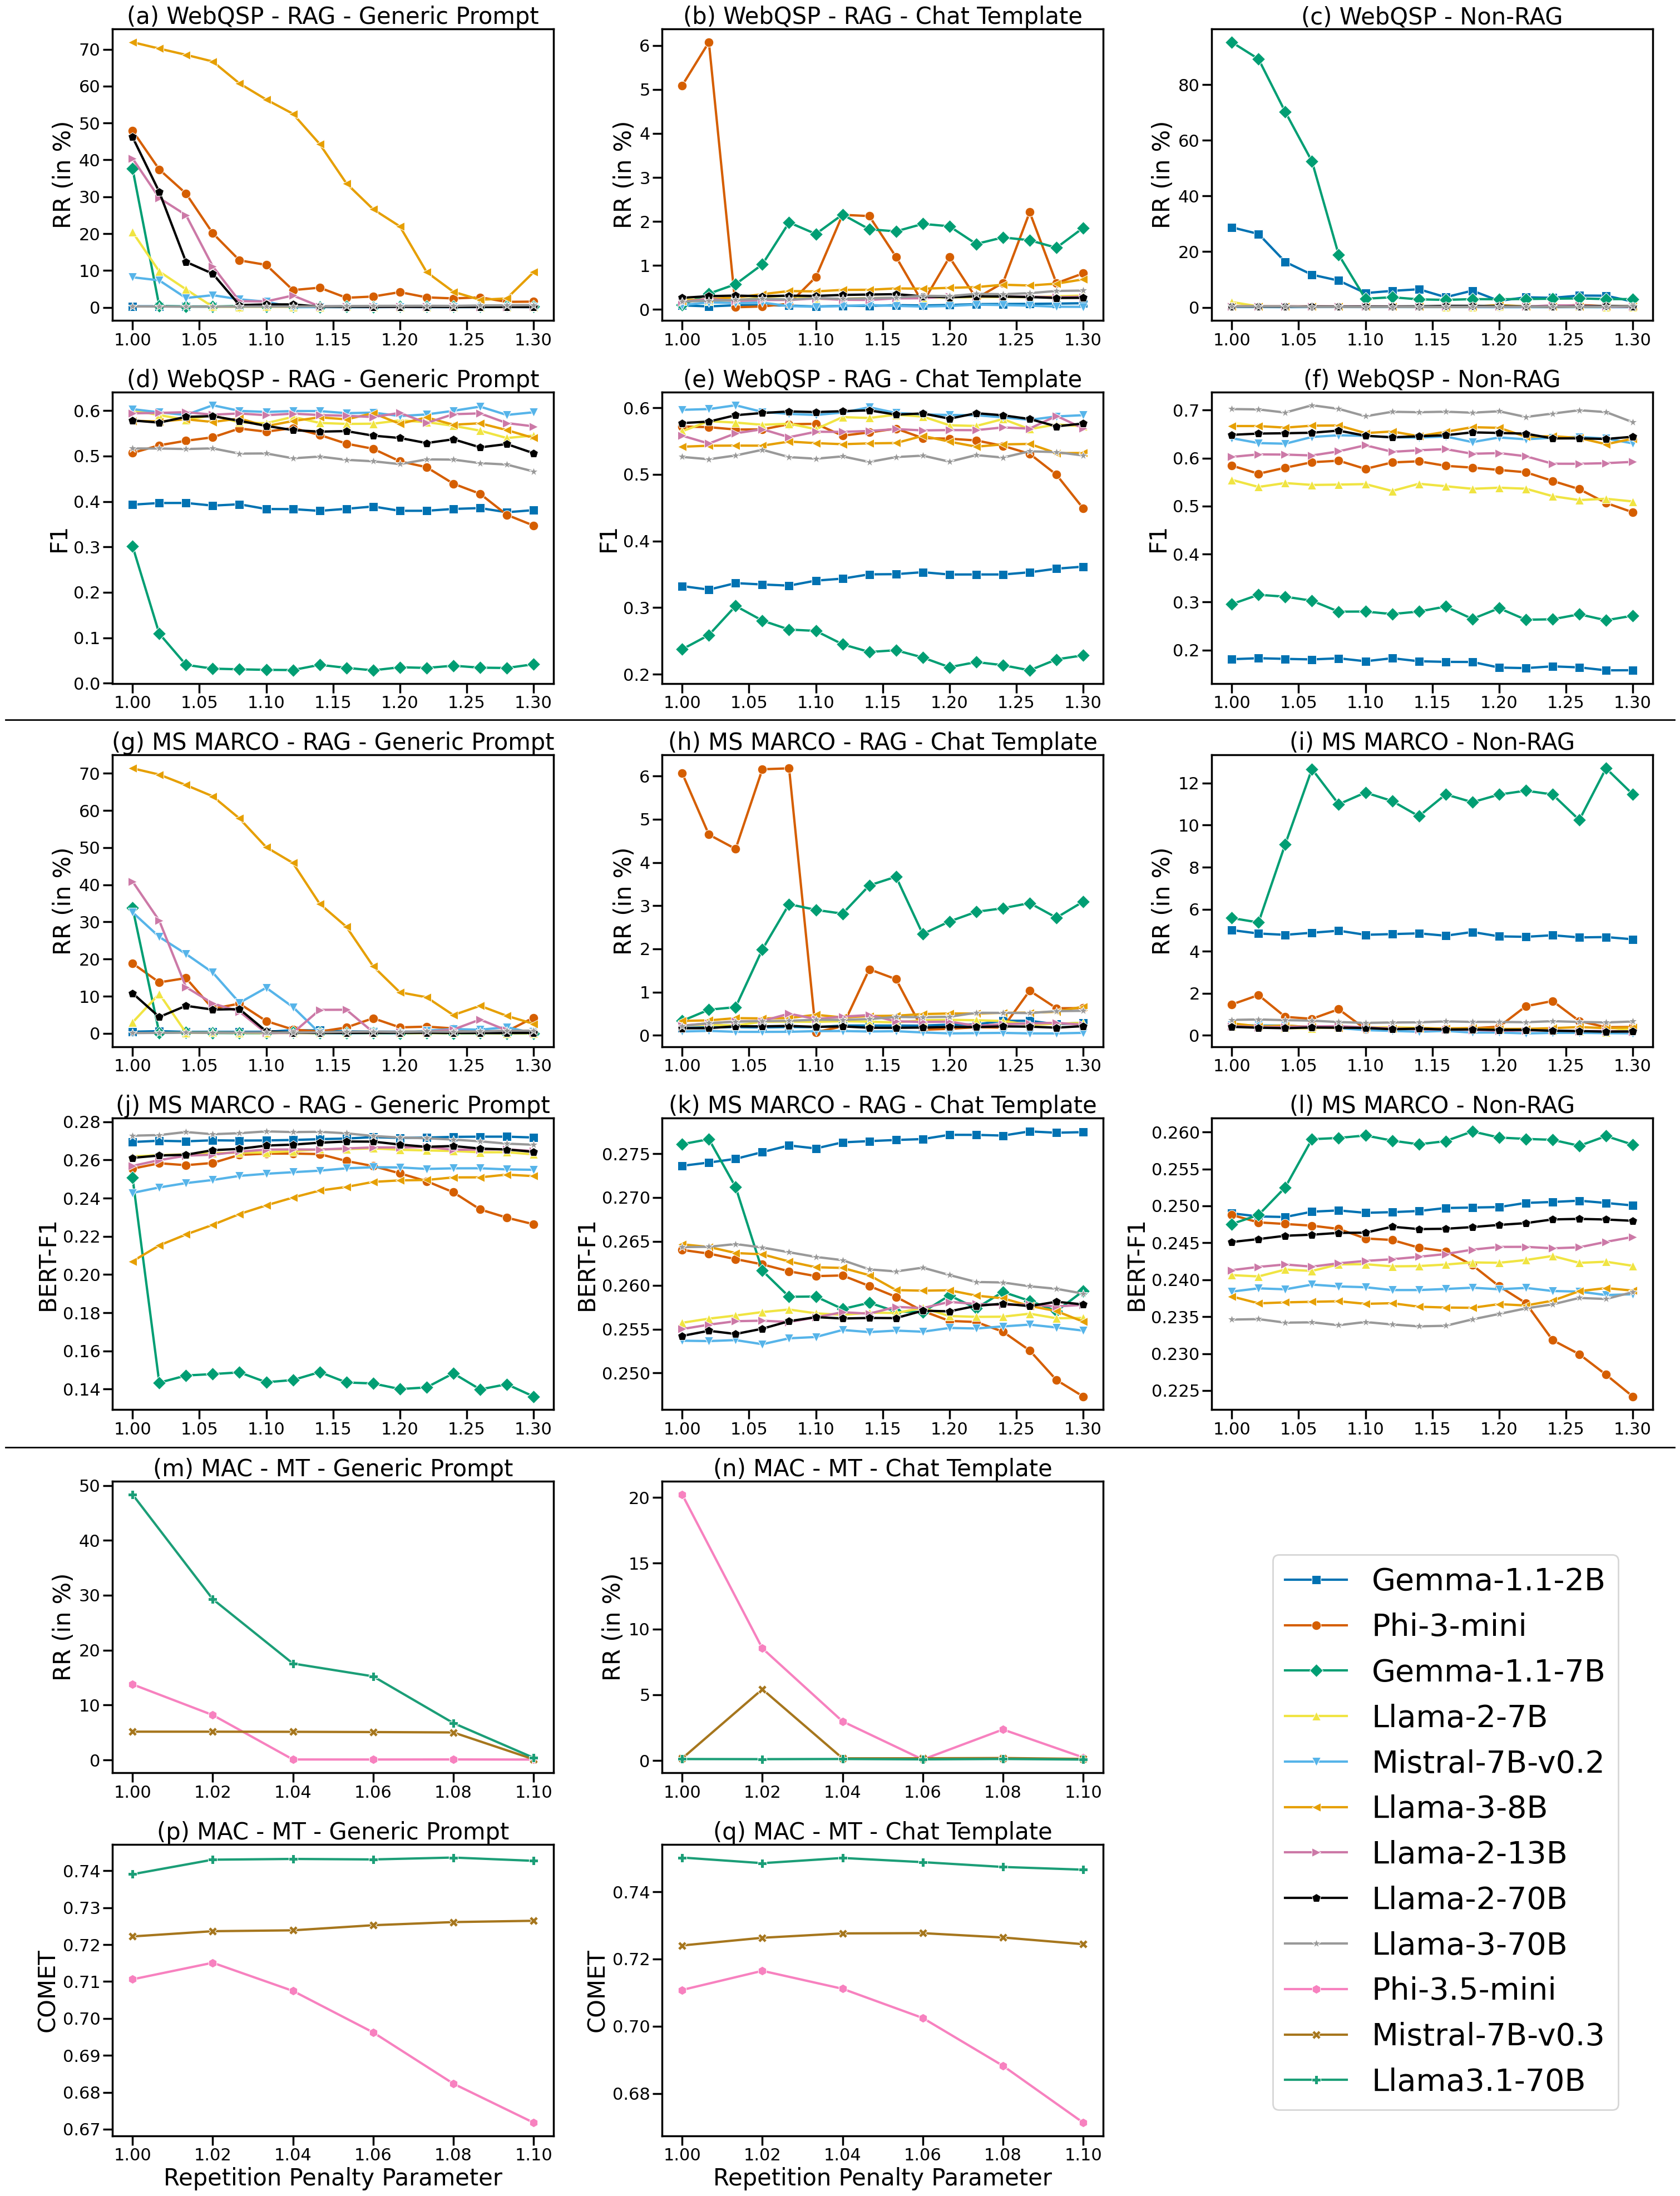
\includegraphics[width=\textwidth]{rap_image/all-metrics-across-models_v2.png}
    \caption{Illustrating the impact of RPP on the repetition ratio (RR) and performance across models, datasets, and prompting strategies.}
    \label{fig:all-metrics-across-models_v2}
\end{figure*}

Figure~\ref{fig:all-metrics-across-models_v2} shows the effect of varying RPP on the repetition and performance of different open-source LLMs across three datasets and multiple prompting strategies. The results indicate that increasing RPP generally reduces repetition; however, this often comes at the expense of performance. The trends and severity vary by model. For example, Phi-3-mini's performance on the MS MARCO dataset drops significantly when RPP exceeds 1.14, whereas Llama-3-8B improves under higher RPP settings. Thus, selecting an optimal RPP is crucial to balance repetition reduction with minimal performance loss.

The datasets also behave differently. WebQSP tends to exhibit higher baseline repetition (e.g., at RPP = 1.0) than MS MARCO, particularly when using the RAG-GP strategy. In the MAC dataset for machine translation, repetition decreases with increasing RPP, even though a smaller range is tested. Notably, for both QA datasets, the Chat Template strategy consistently produces lower RR values compared to the Generic Prompt approach, indicating its effectiveness in minimizing repetition. However, this advantage is not as pronounced in the MT task, where increasing RPP effectively reduces repetition for both prompting strategies.

\subsection{Optimizing the Trade-Off Between Performance and Repetition}
\label{sec:eval_tuning}

\begin{figure*}[htbp]
    \centering
    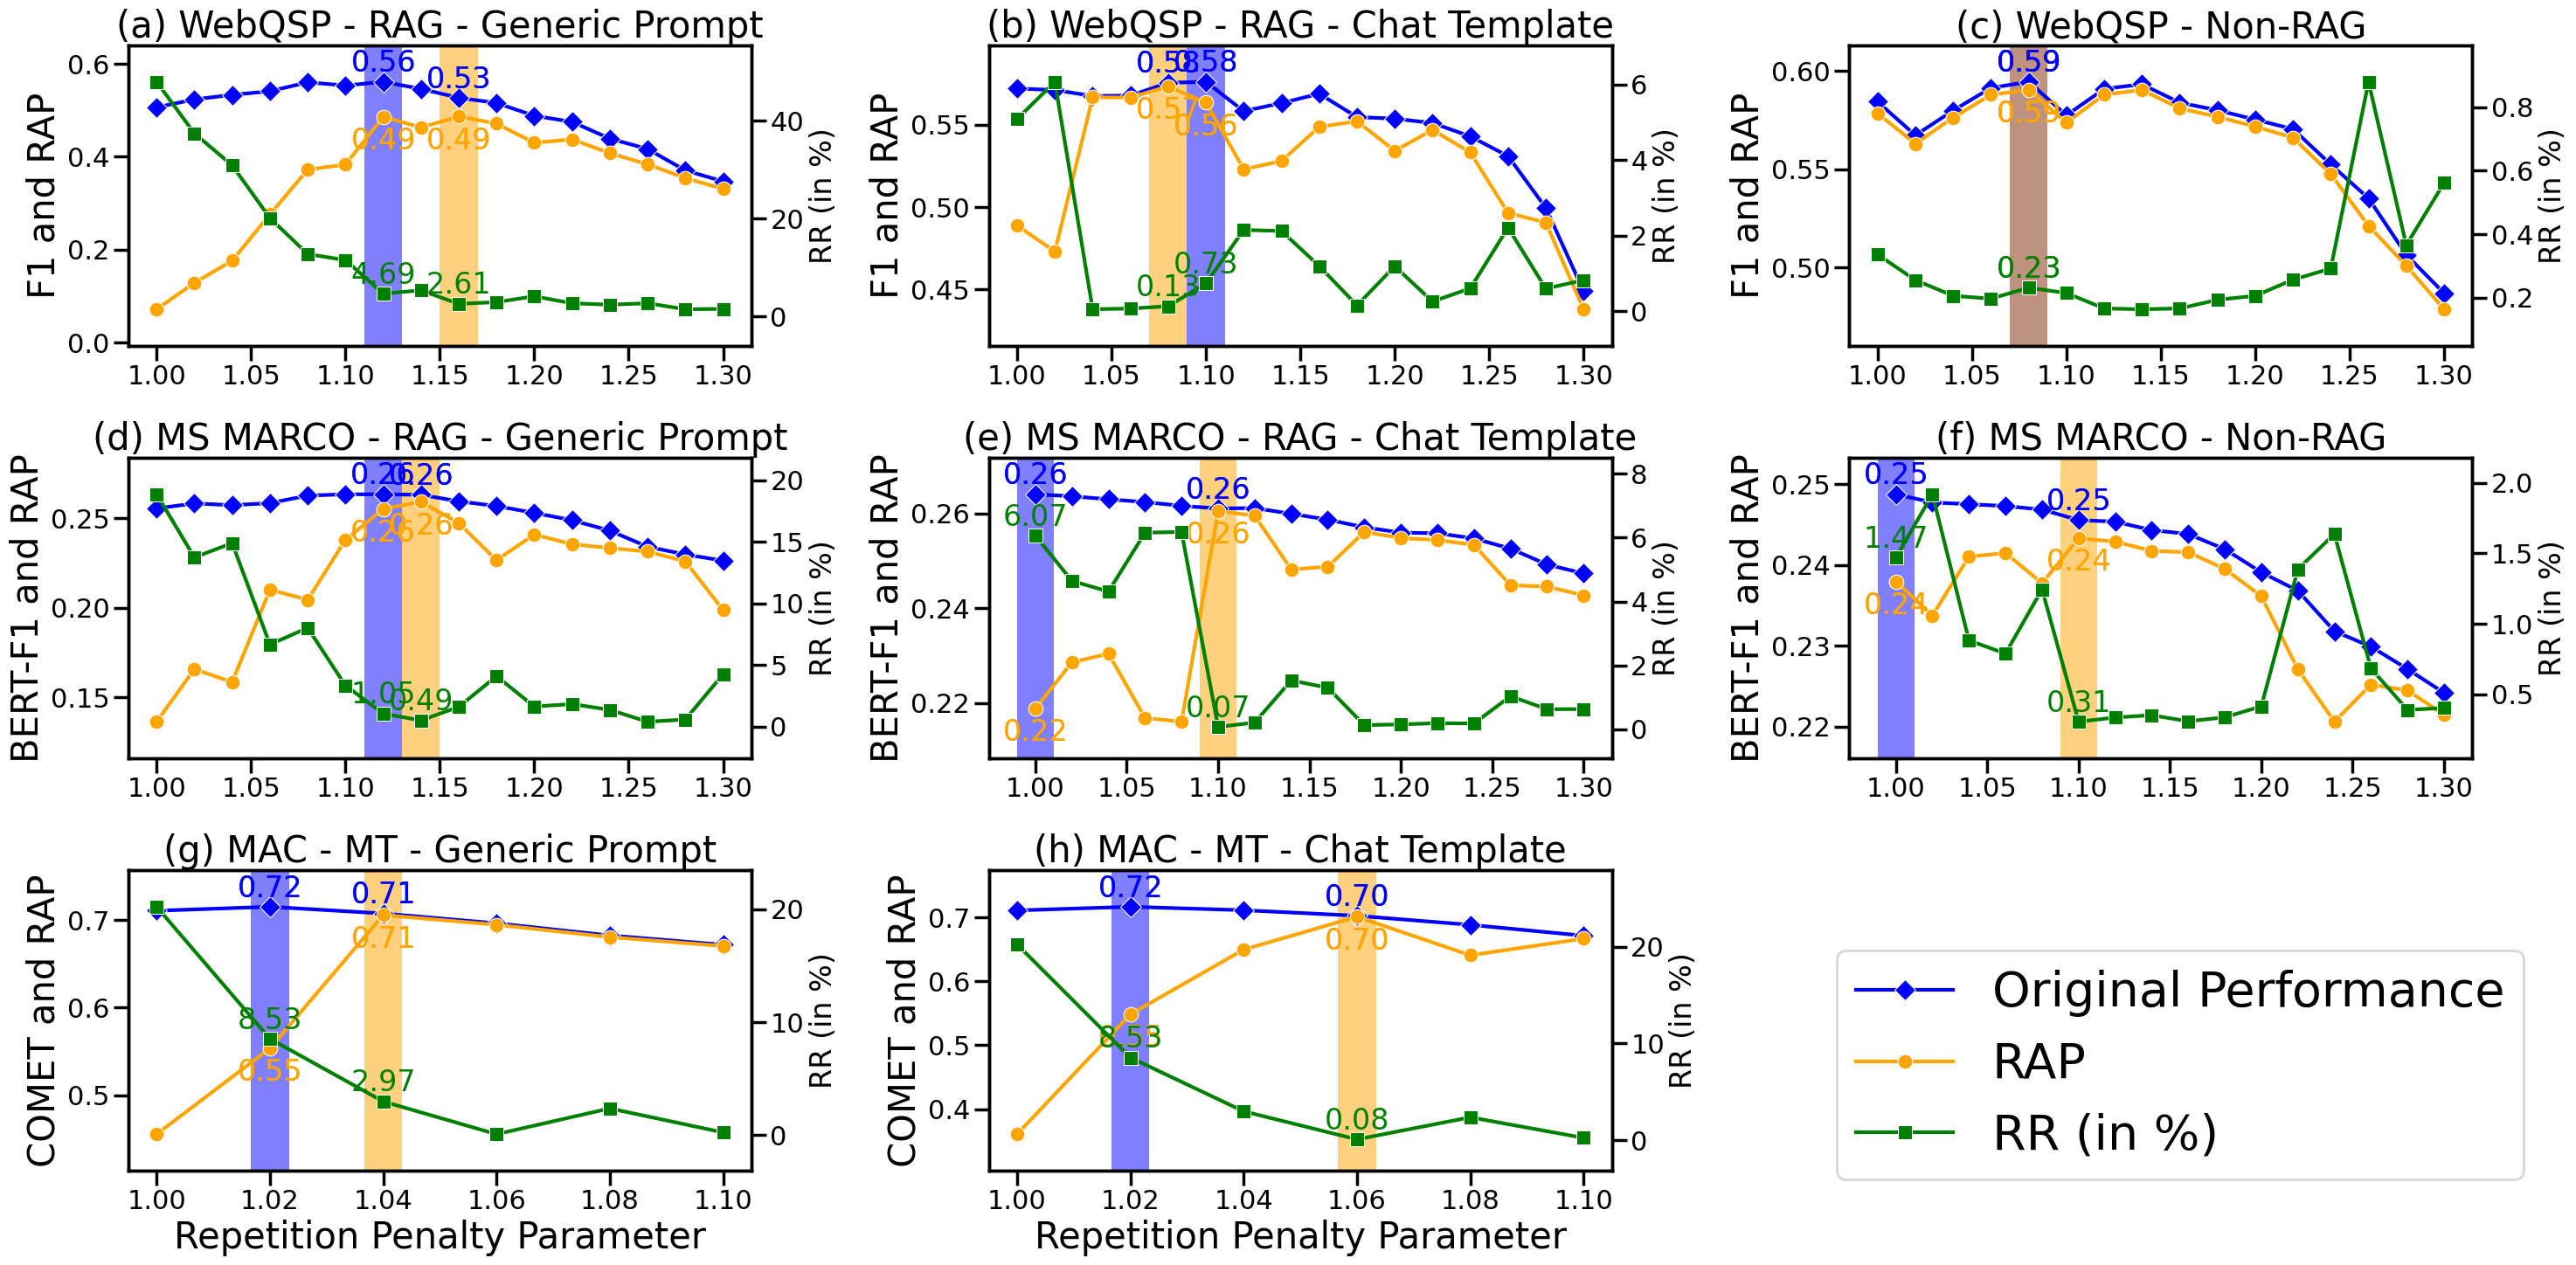
\includegraphics[width=\textwidth]{rap_image/performance_vs_repetition_v2.png}
    \caption{Original performance, repetition-aware performance (RAP), and repetition ratio (RR) for Phi-3-mini in QA (subplots (a) to (f)) and Phi-3.5-mini in MT (subplots (g) and (h)) as a function of RPP. Blue lines represent original performance (F1 for WebQSP, BERT-F1 for MS MARCO, COMET for MAC), orange lines indicate RAP scores, and green lines (right y-axis) show the RR in percentage. The blue shaded region marks the RPP for optimal original performance, the orange region highlights the best RAP, and brown indicates overlap between the two.}
    \label{fig:performance_vs_repetition_v2}
\end{figure*}

This section demonstrates the use of RAP for tuning RPP by comparing conventional performance metrics and repetition-aware performance. Figure~\ref{fig:performance_vs_repetition_v2} presents results for Phi-3-mini on WebQSP and MS MARCO, and for Phi-3.5-mini on MAC. The blue line shows the original performance, the orange line the RAP score, and the green line indicates the repetition ratio (RR). The shaded regions indicate the optimal RPP according to conventional metrics (blue) and RAP (orange); brown shading marks overlapping regions. In most cases (except Figure~\ref{fig:performance_vs_repetition_v2}c), the optimal RPP differs when tuned for original performance versus RAP. For instance, in Figure~\ref{fig:performance_vs_repetition_v2}e, tuning with BERT-F1 yields an optimal RPP of 1.0 with a performance of 0.264 and a high repetition ratio of 6.07\%. With RAP, the optimal RPP shifts to 1.1, where performance drops by only 1.1\% (to 0.261), but the repetition ratio decreases significantly (by about 98.8\%). These results highlight that tuning RPP with RAP better balances performance and repetition reduction.

\subsection{Comparing the RAP-Tuned Performance of All Models}

\begin{table}[htbp]
\centering
\caption{Comparison of model performance across different datasets, LLMs, and prompting strategies.}
\label{tab:model-performance}
\resizebox{.85\columnwidth}{!}{
\begin{tabular}{p{1.2cm}|l|ccc}
\toprule
\multicolumn{1}{l|}{\textbf{Dataset}} & \textbf{LLM} & \textbf{RAG-GP} & \textbf{RAG-CT} & \textbf{Non-RAG} \\ 
\midrule
\multirow{9}{*}{\makecell{WebQSP}} & Gemma-1.1-2B & 0.397 & 0.361 & 0.175 \\
                                   & Phi-3-mini & 0.527 & 0.575 & 0.595 \\
                                   & Gemma-1.1-7B & 0.109 & 0.302 & 0.291 \\
                                   & Mistral-7B-v0.2 & \textbf{0.609} & \textbf{0.604} & 0.648 \\
                                   & Llama-2-7B & 0.589 & 0.590 & 0.548 \\
                                   & Llama-3-8B & 0.572 & 0.558 & 0.668 \\
                                   & Llama-2-13B & 0.595 & 0.588 & 0.627 \\
                                   & Llama-2-70B & 0.577 & 0.596 & 0.657 \\
                                   & Llama-3-70B & 0.517 & 0.537 & \textbf{0.710} \\ 
\midrule
\multirow{9}{*}{\makecell{MS\\MARCO}} & Gemma-1.1-2B & 0.272 & \textbf{0.277} & \textbf{0.250} \\
                                      & Phi-3-mini & 0.263 & 0.261 & 0.246 \\
                                      & Gemma-1.1-7B & 0.149 & 0.276 & 0.249 \\
                                      & Mistral-7B-v0.2 & 0.256 & 0.256 & 0.239 \\
                                      & Llama-2-7B & 0.266 & 0.257 & 0.243 \\
                                      & Llama-3-8B & 0.252 & 0.265 & 0.239 \\
                                      & Llama-2-13B & 0.265 & 0.258 & 0.246 \\
                                      & Llama-2-70B & 0.270 & 0.258 & 0.248 \\
                                      & Llama-3-70B & \textbf{0.275} & 0.264 & 0.238 \\ 
\midrule
\multirow{4}{*}{MAC} & \textbf{LLM} & \textbf{MT-GP} & \textbf{MT-CT} &  \\ \cmidrule{2-5}
                     & Phi-3.5-mini & 0.707 & 0.702 & \\
                     & Mistral-7B-v0.3 & 0.726 & 0.728 & \\
                     & Llama3.1-70B & \textbf{0.743} & \textbf{0.750} & \\ 
\bottomrule
\end{tabular}
}
\end{table}

Table~\ref{tab:model-performance} presents the performance of various open-source LLMs after tuning RPP using RAP. On \textbf{WebQSP}, Mistral-7B leads for both RAG-GP and RAG-CT, scoring 0.609 and 0.604, respectively, while Llama-3-70B achieves the highest F1 of 0.710 in the Non-RAG condition. For \textbf{MS MARCO}, Gemma-1.1-2B excels in both RAG-CT and Non-RAG, with scores of 0.277 and 0.250, respectively, whereas Llama-3-70B attains the best score of 0.275 under RAG-GP. In the MT task (\textbf{MAC}), Llama-3.1-70B outperforms others in both the generic and chat template categories, scoring 0.743 and 0.750. These results demonstrate that larger models like Llama-3-70B and Mistral-7B generally deliver superior performance across datasets and prompting strategies, while mid-sized models like Gemma-1.1-2B can perform competitively on specific tasks. Model choice should therefore be task-dependent rather than based solely on size.

\subsection{How Severe Can Repetition Be?}

\begin{figure}[htbp]
    \centering
    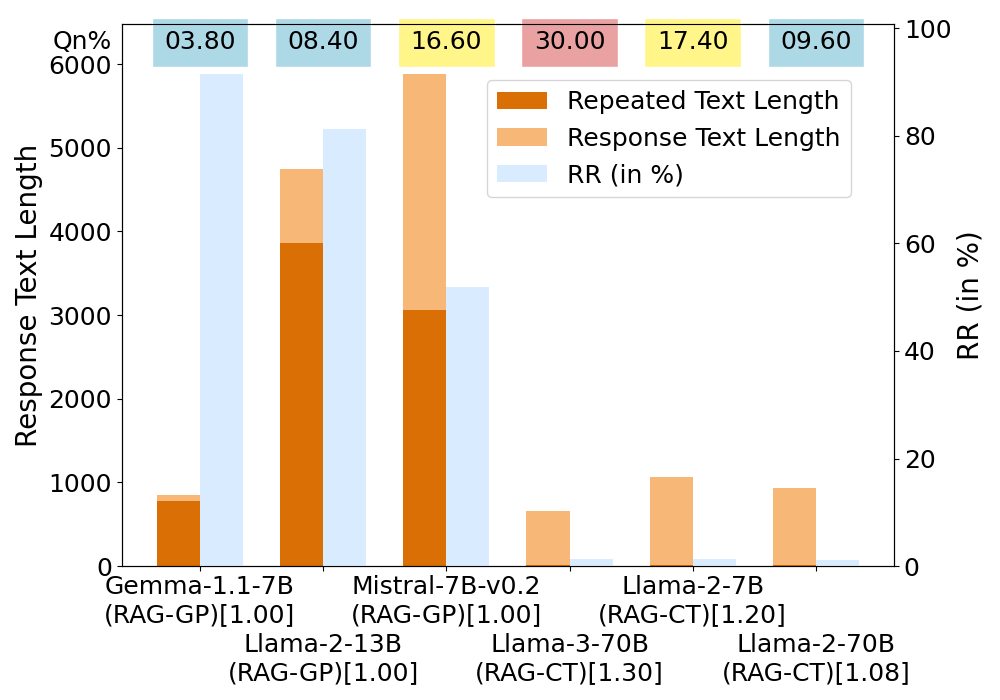
\includegraphics[width=1\linewidth]{rap_image/chart_02_mm.png}
    \caption{Severity of repetition. Colored squares above each point indicate the percentage of repetitive responses. The x-axis labels include the model, prompting method, and tuned RPP value.}
    \label{fig:msmarco_top3}
\end{figure}

In our experiments, repeated text can account for up to 97.85\% of the overall output, and up to 41.27\% of responses exhibit repetition. Figure~\ref{fig:msmarco_top3} shows the three highest and three lowest repetition ratios (RR) for the MS MARCO dataset. Colored squares above each point indicate the percentage of repeated responses (blue: below 10\%, yellow: 10--20\%, red: above 20\%). Notably, while Gemma-1.1-7B (RAG-GP) shows only 3.8\% of responses with repetition, in those cases the repeated text makes up 91.53\% of the total output length. In contrast, although 30\% of Llama-3-70B (RAG-CT)'s responses contain repetition, the repeated text comprises only 1.29\% of the overall length. For example, Llama-2-13B generated repeated content averaging around 4,000 characters.

These severity findings underscore the importance of addressing repetition not only for user experience but also for downstream system reliability. In multi-agent systems (Chapter~\ref{ch:agentic}), repetitive outputs from one agent can propagate errors through the pipeline, degrading overall workflow success rates. The RAP metric thus serves as both an evaluation tool and a quality gate for production deployments.

\subsection{Ablation Study: Effects of Different Penalty Functions}

\begin{figure}[htbp]
    \centering
    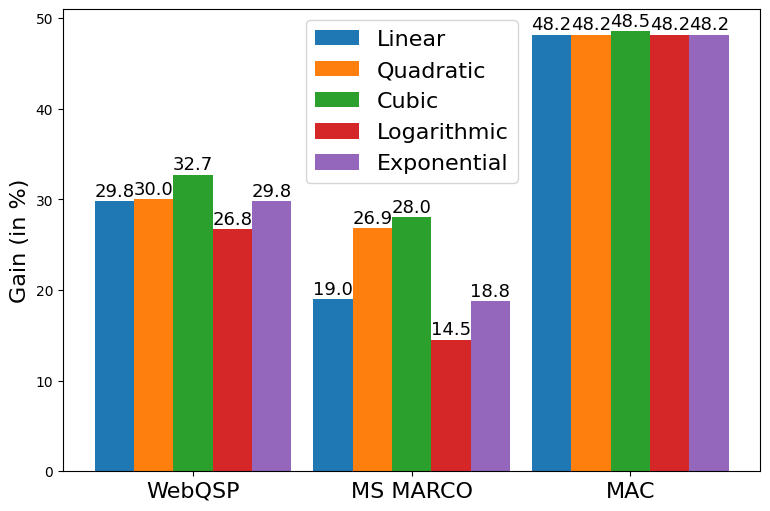
\includegraphics[width=\linewidth]{rap_image/ablation_study.png}
    \caption{Gains across different penalty functions. The \textit{Cubic} penalty consistently achieves the highest gains across all three datasets.}
    \label{fig:ablation_study}
\end{figure}

We present an ablation study to evaluate the impact of different penalty functions $F(\text{RR})$ on the RAP metric (Equation~\ref{eq:rap}). We consider five options:
\begin{itemize}[leftmargin=*]
    \item \textit{Linear}: $F(\text{RR})=1-\text{RR}$,
    \item \textit{Quadratic}: $F(\text{RR})=(1-\text{RR})^2$,
    \item \textit{Cubic}: $F(\text{RR})=(1-\text{RR})^3$,
    \item \textit{Logarithmic}: $F(\text{RR})=\log_{2}(2-\text{RR})$,
    \item \textit{Exponential}: $F(\text{RR})=e^{-\text{RR}}$.
\end{itemize}

We compare the \textit{Gain} achieved with each penalty formula. For a given model, \textit{Gain} is defined as the difference between the reduction in repetition and the performance drop when tuning the repetition penalty parameter (RPP) using original performance metrics versus RAP. In other words, it reflects the relative decrease in repetition compared to the loss in performance; a higher \textit{Gain} indicates a more favorable trade-off.

Figure~\ref{fig:ablation_study} shows the average \textit{Gain} scores for each penalty function across the three datasets, computed by averaging the gains from all models and prompting strategies. The results indicate that the \textit{Cubic} penalty consistently yields the highest gains (32.7\% for WebQSP, 28.0\% for MS MARCO, and 48.5\% for MAC), offering the best balance between reducing repetition and maintaining performance. These findings recommend the \textit{Cubic} penalty for the RAP metric across diverse datasets and tasks.

\subsection{Summary of RAP Findings}

This research tackles the challenge of reducing repeated content generation while preserving overall performance in open-source LLMs. We propose the repetition-aware performance metric, RAP, which quantifies and integrates repetition penalty into model evaluation. Conventional metrics often overlook repetition, making it difficult to tune the repetition penalty parameter (RPP). In contrast, RAP enables effective tuning of RPP and can be easily applied to other repetition methods as well.

We evaluated RAP on twelve open-source LLMs using three datasets across QA and MT tasks, with different prompting strategies. Results show that higher RPP values generally reduce repetition but can significantly impact performance. This phenomenon emphasizes the need for tuning RPP. 
The experiments also demonstrate the capability of using RAP for identifying the RPP value that efficiently reduces repetition while minimizing performance loss.
We also highlight the severity of the repetition issues in the generated content, calling for greater attention from the research community on this matter.
Our experiments offer valuable insights into managing repetition in open-source LLMs, including a recommendation to use Chat Templates for RAG prompting.

The RAP methodology---combining detection, quantification, and penalty-based optimization---exemplifies the evaluation framework philosophy that permeates this dissertation. Just as RAP integrates output quality into traditional performance metrics, the Agentic Success Rate (Chapter~\ref{ch:agentic}) integrates pipeline reliability into task completion metrics, and the Reasoning Intensity metric (Chapter~\ref{ch:strategies}) integrates computational efficiency into accuracy assessment. This pattern of multi-dimensional evaluation addresses the fundamental insight that single-metric optimization yields systems that perform well on benchmarks but poorly in production.

\section{Evaluation-Guided Hyperparameter Search}
\label{sec:rag_opt}

Building on our prior work---including our NAACL 2025 paper on the RAP metric---we propose an evaluation-guided hyperparameter search loop for optimizing Retrieval-Augmented Generation (RAG) systems. The workflow is detailed in Algorithm~\ref{alg:hyperparameter_search}.

\begin{algorithm}[htbp]
\caption{Hyperparameter Search for RAG Optimization}
\label{alg:hyperparameter_search}
\begin{algorithmic}[1]
\Require Validation set $Q$ of queries (with ground-truth answers), initial retriever and LLM, and search space $\Lambda$ for hyperparameters (e.g., retrieval and generation settings).
\Ensure Optimal hyperparameter setting $\lambda^*$.
\For{each candidate setting $\lambda \in \Lambda$ (or using an intelligent search strategy)}
    \State Configure the retriever/LLM with $\lambda$ (e.g., set $k$, $\tau$, RPP, etc.)
    \State Generate answers $\hat{Y} = \{\hat{y}_q : q \in Q\}$ using the RAG pipeline
    \State Evaluate $\hat{Y}$ against ground truth $Y$ to obtain a performance score $P(\hat{Y}, Y)$ (e.g., average accuracy or F1)
    \State Compute repetition or other penalties $R(\hat{Y})$ (e.g., repetition ratio)
    \State Compute the overall metric $M(\hat{Y})$, which combines performance and penalties (e.g., the RAP score as in Equation~\ref{eq:rap})
    \State Record $(\lambda, M(\hat{Y}))$
\EndFor
\State \textbf{return} $\lambda^* = \arg\max_{\lambda} M(\hat{Y}_\lambda)$
\end{algorithmic}
\end{algorithm}

In this procedure, the search space $\Lambda$ may be explored exhaustively or using an intelligent algorithm. The metric $M$ can be defined as the standard performance metric $P$ if accuracy is the only concern, but it is often augmented to incorporate aspects such as brevity or non-repetition. Our proposed RAP metric (see Section~\ref{sec:rap_definition}) is one such example. By using RAP as the optimization target, configurations that yield correct yet non-repetitive outputs are inherently favored.

In our work, this approach is used to tune the repetition penalty parameter (RPP). Traditional grid search using only accuracy would not differentiate between two configurations with similar accuracy but differing levels of verbosity. By contrast, an augmented metric like RAP can prioritize configurations with lower redundancy. We also verify that the final chosen $\lambda^*$ is robust, using a separate test set or cross-validation.

It is important to note that hyperparameter choices may interact. For example, extensive fine-tuning of the LLM may alter its sensitivity to decoding parameters, and a stronger retriever (providing higher quality documents) may permit a lower repetition penalty. Thus, hyperparameter optimization is an ongoing process that evolves with model development.

In conclusion, the RAP metric offers a nuanced evaluation of RAG systems, particularly when optimizing open-source LLMs prone to repetition. By integrating RAP into our development cycle, we ensure that our optimized RAG system retrieves and generates correct information in a succinct and user-friendly manner. Future work may extend RAP to include additional factors (e.g., factuality or coherence), but as a first step, it significantly enhances our ability to mitigate a common failure mode in open-source LLM generation.

\section{Practical Deployment Guidelines}
\label{sec:rag_guidelines}

Based on our comprehensive evaluation, we synthesize the following guidelines for enterprise RAG deployment:

\textbf{Model Selection.} Open-source models such as Orca-2 and Mistral-7B can achieve generation quality competitive with proprietary alternatives while offering significant advantages in deployment flexibility, cost, and data privacy. Orca-2-13b achieved 99.3\% overall RAGAS score, surpassing GPT-4 (97.5\%) while operating on consumer-grade hardware. For RAG applications requiring high faithfulness, models specifically trained to follow retrieved context (rather than relying on parametric knowledge) should be prioritized.

\textbf{Hardware Planning.} Model size should be matched to available hardware:
\begin{itemize}[leftmargin=*]
    \item 7B-parameter models perform efficiently on consumer GPUs (RTX 4090, 24GB VRAM), achieving approximately 33 tokens/second
    \item 13B+ models benefit substantially from professional-grade hardware (A40, L40 with 48GB VRAM) or cloud deployment
    \item Memory capacity is the primary constraint for larger models; insufficient VRAM leads to significant performance degradation
\end{itemize}
These hardware findings inform the comprehensive edge deployment evaluation in Chapter~\ref{ch:strategies}, where we extend benchmarking across six hardware platforms.

\textbf{Repetition Management.} The repetition penalty parameter (RPP) should be systematically tuned using RAP rather than default values:
\begin{itemize}[leftmargin=*]
    \item RAP-guided tuning achieves up to 93.1\% repetition reduction with only 3.7\% performance degradation
    \item The cubic penalty function $F(\text{RR}) = (1-\text{RR})^3$ provides optimal balance across datasets
    \item Chat templates consistently reduce repetition compared to generic prompts in RAG configurations
    \item Optimal RPP varies substantially across models and datasets---Phi-3-mini degrades sharply above RPP 1.14, while Llama-3-8B improves
\end{itemize}

\textbf{Evaluation Strategy.} Employ multi-dimensional evaluation combining faithfulness, relevance, and repetition metrics. Single-metric optimization may yield configurations that perform well on benchmarks but poorly in practice. The RAP framework demonstrates this principle: optimizing for accuracy alone selects configurations with high redundancy, while RAP-guided optimization achieves comparable accuracy with dramatically reduced repetition.

\textbf{Prompt Engineering.} Prompt template selection significantly impacts both retrieval quality and generation coherence:
\begin{itemize}[leftmargin=*]
    \item Chat templates reduce repetition and improve context utilization
    \item Model-specific templates (respecting each model's expected format) outperform generic prompts
    \item Standalone question generation quality affects retrieval relevance---models producing generic questions may retrieve suboptimal context
\end{itemize}

\section{Summary}

This chapter presented a comprehensive framework for optimizing Retrieval-Augmented Generation (RAG) systems built on open-source Large Language Models. Drawing from three accepted publications, we addressed the critical challenges of model selection, evaluation methodology, and generation quality that enterprises face when deploying RAG solutions.

Our comparative evaluation of LLMs on the PCI DSS benchmark revealed that smaller, efficient models such as Orca-2-13b can achieve generation quality competitive with---or exceeding---proprietary alternatives like GPT-4, while maintaining practical inference speeds on consumer-grade hardware. Specifically, Orca-2-13b achieved a 99.3\% overall RAGAS score with perfect faithfulness, demonstrating that model size alone does not determine RAG effectiveness. This finding---that architecture and training methodology matter more than scale---recurs throughout this dissertation and informs model selection strategies in subsequent chapters.

Central to our contribution is the Repetition-Aware Performance (RAP) metric, which addresses a pervasive yet overlooked problem in open-source LLM outputs: excessive repetition. Through systematic evaluation of twelve models across question answering and machine translation tasks, we demonstrated that repeated content can comprise over 90\% of generated text in severe cases, with up to 41\% of responses exhibiting redundancy. The RAP metric integrates a cubic penalty function that enables principled tuning of the repetition penalty parameter (RPP), achieving up to 93.1\% reduction in repetition with minimal performance degradation (typically under 4\%). Cross-task validation on machine translation confirmed RAP's generalizability beyond RAG-specific applications.

Our experimental analysis yielded several practical insights for enterprise deployment. Chat templates significantly reduce repetition compared to generic prompts in RAG configurations, providing a simple yet effective mitigation strategy. The optimal RPP varies substantially across models and datasets, underscoring the importance of systematic hyperparameter tuning rather than default settings. Additionally, hardware memory capacity critically impacts performance for larger models, with the RTX 4090 supporting efficient inference for 7B-parameter models while 13B models benefit substantially from professional-grade GPUs like the A40.

The evaluation-guided hyperparameter search procedure presented in this chapter operationalizes these findings, using RAP as the optimization target to identify configurations that balance factual accuracy, relevance, and output conciseness. This holistic approach ensures that optimized RAG systems not only retrieve and generate correct information but deliver it in a manner suitable for enterprise applications where user experience and response clarity are paramount.

The methodological contributions of this chapter---particularly the philosophy of multi-dimensional evaluation that integrates quality considerations beyond accuracy---establish foundations for subsequent chapters. Chapter~\ref{ch:agentic} extends this approach to multi-agent systems with the Agentic Success Rate (ASR) and Evaluation Completion Rate (ECR@1), while Chapter~\ref{ch:strategies} applies similar principles through Reasoning Intensity (RI) and domain-specific metrics for translation and predictive analytics.